% ============================================================
\chapter{Applied Graph Theory}
\label{ch:graphs}
% ============================================================

In 1736, Leonhard Euler turned his attention to a recreational problem posed by the inhabitants of K\"onigsberg: is it possible to cross the city's seven bridges, passing over each one exactly once? By proving that it is impossible, Euler did not merely solve a puzzle about walks: he founded graph theory, a branch of mathematics that would become indispensable to operations research. Today, graphs model transportation networks, electronic circuits, social networks, and supply chains. Finding the shortest path, the minimum spanning tree, the maximum flow --- these fundamental problems have algorithms (Dijkstra, Kruskal, Ford-Fulkerson) that are executed millions of times daily in computer systems around the world.

\section{Fundamental definitions}

\begin{definition}[Graph]
A \textbf{graph} $G = (V, E)$ is a pair where $V$ is a finite set of
\textbf{vertices} (or nodes) and $E$ is a set of \textbf{edges} (undirected
graph) or \textbf{arcs} (directed graph, denoted $G = (V, A)$).
\end{definition}

\begin{definition}[Weighted graph]
A graph is \textbf{weighted} if each edge/arc $(i,j)$ is endowed with a weight
$w(i,j) \in \R$ (distance, cost, capacity, etc.).
\end{definition}

\begin{center}
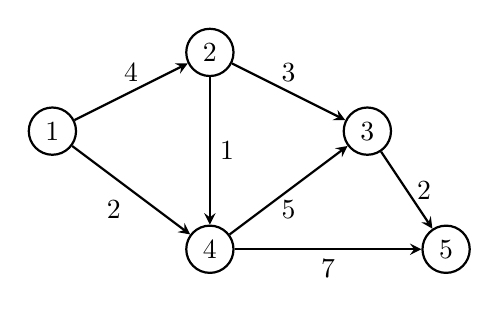
\begin{tikzpicture}[
    vertex/.style={circle, draw, minimum size=6mm, inner sep=0pt},
    >=stealth, thick
  ]
  \node[vertex] (1) at (0,2) {1};
  \node[vertex] (2) at (2,3) {2};
  \node[vertex] (3) at (4,2) {3};
  \node[vertex] (4) at (2,0.5) {4};
  \node[vertex] (5) at (5,0.5) {5};
  \draw[->] (1) -- node[above] {4} (2);
  \draw[->] (1) -- node[below left] {2} (4);
  \draw[->] (2) -- node[above] {3} (3);
  \draw[->] (2) -- node[right] {1} (4);
  \draw[->] (3) -- node[right] {2} (5);
  \draw[->] (4) -- node[below] {5} (3);
  \draw[->] (4) -- node[below] {7} (5);
\end{tikzpicture}
\end{center}

\begin{definition}[Path and cycle]
A \textbf{path} from $u$ to $v$ is a sequence of vertices
$u = v_0, v_1, \ldots, v_k = v$ such that $(v_{i-1}, v_i) \in E$ for all $i$.
Its \textbf{length} is the sum of the weights. A \textbf{cycle} is a closed
path ($u = v$) of nonzero length.
\end{definition}

\begin{definition}[Connected graph]
An undirected graph is \textbf{connected} if there exists a path between every
pair of vertices. A directed graph is \textbf{strongly connected} if there
exists a directed path between every ordered pair of vertices.
\end{definition}

\begin{definition}[Tree]
A \textbf{tree} is a connected graph without cycles. It has exactly
$\abs{V} - 1$ edges.
\end{definition}

\section{Graph representations}

\begin{keyformulas}[title=\textbf{Data structures}]
\begin{itemize}
  \item \textbf{Adjacency matrix} $A \in \{0,1\}^{n \times n}$:
        $A_{ij} = 1$ if $(i,j) \in E$. Memory: $\mathcal{O}(n^2)$.
  \item \textbf{Adjacency lists}: for each vertex, the list of its neighbors.
        Memory: $\mathcal{O}(n + m)$.
  \item \textbf{Weight matrix} $W$: $W_{ij} = w(i,j)$ or $+\infty$ if
        $(i,j) \notin E$.
\end{itemize}
\end{keyformulas}

\section{Single-source shortest paths}

\subsection{Dijkstra's algorithm}

\begin{theorem}[Dijkstra's correctness]
\index{Dijkstra's algorithm}
Dijkstra's algorithm computes shortest paths from a source vertex $s$ in a
graph with \textbf{nonnegative} weights in time $\mathcal{O}((n + m) \log n)$
using a binary heap.
\end{theorem}

\begin{algorithme}[title=\textbf{Dijkstra's Algorithm}]
\begin{enumerate}
  \item Initialize $d[s] = 0$, $d[v] = +\infty$ for $v \ne s$.
  \item $Q \leftarrow V$ (priority queue).
  \item While $Q \ne \emptyset$:
    \begin{enumerate}
      \item Extract $u = \argmin_{v \in Q} d[v]$.
      \item For each neighbor $v$ of $u$ with $(u,v) \in E$:
        if $d[u] + w(u,v) < d[v]$:
        $d[v] \leftarrow d[u] + w(u,v)$, $\pi[v] \leftarrow u$.
    \end{enumerate}
\end{enumerate}
\end{algorithme}

\begin{example}[Dijkstra]
On the graph above with source $s = 1$:

\begin{center}
\begin{tabular}{c|ccccc}
  Step & $d[1]$ & $d[2]$ & $d[3]$ & $d[4]$ & $d[5]$ \\
  \hline
  Init & 0 & $\infty$ & $\infty$ & $\infty$ & $\infty$ \\
  $u=1$ & 0 & 4 & $\infty$ & 2 & $\infty$ \\
  $u=4$ & 0 & 3 & 7 & 2 & 9 \\
  $u=2$ & 0 & 3 & 6 & 2 & 9 \\
  $u=3$ & 0 & 3 & 6 & 2 & 8 \\
  $u=5$ & 0 & 3 & 6 & 2 & 8 \\
\end{tabular}
\end{center}

Shortest path $1 \to 5$: $1 \to 4 \to 3 \to 5$ of length 8.
\end{example}

\subsection{Bellman-Ford algorithm}

\begin{theorem}[Bellman-Ford]
\index{Bellman-Ford algorithm}
The Bellman-Ford algorithm computes shortest paths from $s$ in the presence of
\textbf{negative} weights (but no reachable negative cycle) in time
$\mathcal{O}(nm)$.
\end{theorem}

\begin{algorithme}[title=\textbf{Bellman-Ford Algorithm}]
\begin{enumerate}
  \item Initialize $d[s] = 0$, $d[v] = +\infty$ for $v \ne s$.
  \item Repeat $\abs{V} - 1$ times:
    \begin{enumerate}
      \item For each arc $(u,v) \in A$: if $d[u] + w(u,v) < d[v]$:
            $d[v] \leftarrow d[u] + w(u,v)$, $\pi[v] \leftarrow u$.
    \end{enumerate}
  \item \textbf{Negative cycle detection}: for each arc $(u,v)$:
        if $d[u] + w(u,v) < d[v]$, a negative cycle exists.
\end{enumerate}
\end{algorithme}

\begin{warning}[title=\textbf{Negative cycles}]
In the presence of a negative cycle reachable from $s$, shortest paths are
undefined (distances can go to $-\infty$). Bellman-Ford detects this situation.
\end{warning}

\section{All-pairs shortest paths}

\begin{algorithme}[title=\textbf{Floyd-Warshall Algorithm}]
\index{Floyd-Warshall algorithm}
Complexity: $\mathcal{O}(n^3)$.
\begin{enumerate}
  \item Initialize $D^{(0)} = W$ (weight matrix).
  \item For $k = 1, \ldots, n$:
    \[
      D^{(k)}_{ij} = \min\left(D^{(k-1)}_{ij},\;
        D^{(k-1)}_{ik} + D^{(k-1)}_{kj}\right)
    \]
\end{enumerate}
\end{algorithme}

\section{Minimum spanning trees}

\begin{definition}[Minimum spanning tree (MST)]
\index{minimum spanning tree}
A \textbf{minimum spanning tree} of a connected weighted graph $G = (V, E)$ is
a spanning subgraph without cycles of minimum total weight.
\end{definition}

\subsection{Kruskal's algorithm}

\begin{algorithme}[title=\textbf{Kruskal's Algorithm}]
\index{Kruskal's algorithm}
\begin{enumerate}
  \item Sort edges by increasing weight.
  \item For each edge $(u,v)$ in weight order:
    \begin{enumerate}
      \item If $u$ and $v$ are in different components: add $(u,v)$ to the MST
            and merge the components (Union-Find).
    \end{enumerate}
  \item Stop after $\abs{V} - 1$ edges.
\end{enumerate}
Complexity: $\mathcal{O}(m \log m)$.
\end{algorithme}

\subsection{Prim's algorithm}

\begin{algorithme}[title=\textbf{Prim's Algorithm}]
\index{Prim's algorithm}
\begin{enumerate}
  \item Choose an initial vertex $s$. $T \leftarrow \{s\}$.
  \item While $\abs{T} < \abs{V}$:
    \begin{enumerate}
      \item Find the minimum-weight edge $(u,v)$ with $u \in T$, $v \notin T$.
      \item Add $v$ to $T$ and $(u,v)$ to the MST.
    \end{enumerate}
\end{enumerate}
Complexity: $\mathcal{O}((n + m) \log n)$ with a binary heap.
\end{algorithme}

\begin{example}[MST by Kruskal]
\begin{center}
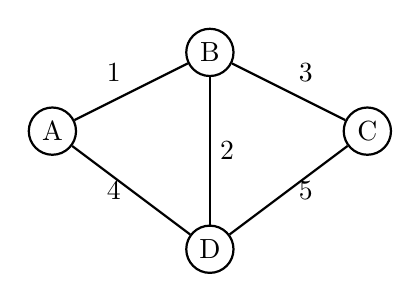
\begin{tikzpicture}[
    vertex/.style={circle, draw, minimum size=6mm, inner sep=0pt},
    thick
  ]
  \node[vertex] (A) at (0,2) {A};
  \node[vertex] (B) at (2,3) {B};
  \node[vertex] (C) at (4,2) {C};
  \node[vertex] (D) at (2,0.5) {D};
  \draw (A) -- node[above left] {1} (B);
  \draw (A) -- node[left] {4} (D);
  \draw (B) -- node[above right] {3} (C);
  \draw (B) -- node[right] {2} (D);
  \draw (C) -- node[right] {5} (D);
\end{tikzpicture}
\end{center}

Sorted edges: $(A,B)=1$, $(B,D)=2$, $(B,C)=3$, $(A,D)=4$, $(C,D)=5$.

MST: $\{(A,B), (B,D), (B,C)\}$, total weight $= 1 + 2 + 3 = 6$.
\end{example}

\section{Python implementation with NetworkX}

\begin{codeblock}[title=\textbf{Shortest paths and MST}]
\begin{minted}{python}
import networkx as nx

# Create directed graph
G = nx.DiGraph()
edges = [(1,2,4), (1,4,2), (2,3,3), (2,4,1),
         (3,5,2), (4,3,5), (4,5,7)]
G.add_weighted_edges_from(edges)

# Dijkstra
dist, path = nx.single_source_dijkstra(G, source=1)
print("Distances from 1:", dist)
print("Path 1->5:", path[5])

# Bellman-Ford
dist_bf = nx.single_source_bellman_ford_path_length(G, 1)
print("Bellman-Ford:", dict(dist_bf))

# Undirected graph for MST
H = nx.Graph()
H.add_weighted_edges_from([
    ('A','B',1), ('A','D',4), ('B','C',3),
    ('B','D',2), ('C','D',5)
])

mst = nx.minimum_spanning_tree(H, algorithm='kruskal')
print("\nMST (Kruskal):")
for u, v, d in mst.edges(data=True):
    print(f"  {u}--{v} : {d['weight']}")
print(f"Total weight: {sum(d['weight']
       for _,_,d in mst.edges(data=True))}")
\end{minted}
\end{codeblock}

\section{Applications}

\begin{itemize}
  \item \textbf{GPS and navigation}: shortest paths (Dijkstra, $A^*$).
  \item \textbf{Telecommunications}: MST for optimal cabling.
  \item \textbf{Project planning}: PERT/CPM (critical path = longest path in
        a DAG).
  \item \textbf{Scheduling}: topological sort in a precedence graph.
\end{itemize}

\section{Exercises}

\begin{exercise}[$\star$ -- Dijkstra]
Apply Dijkstra to the following graph from vertex $A$:

\begin{center}
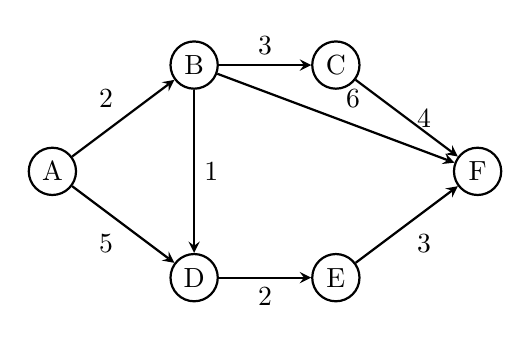
\begin{tikzpicture}[
    vertex/.style={circle, draw, minimum size=6mm, inner sep=0pt},
    >=stealth, thick, scale=0.9
  ]
  \node[vertex] (A) at (0,1.5) {A};
  \node[vertex] (B) at (2,3) {B};
  \node[vertex] (C) at (4,3) {C};
  \node[vertex] (D) at (2,0) {D};
  \node[vertex] (E) at (4,0) {E};
  \node[vertex] (F) at (6,1.5) {F};
  \draw[->] (A) -- node[above left] {2} (B);
  \draw[->] (A) -- node[below left] {5} (D);
  \draw[->] (B) -- node[above] {3} (C);
  \draw[->] (B) -- node[right] {1} (D);
  \draw[->] (C) -- node[right] {4} (F);
  \draw[->] (D) -- node[below] {2} (E);
  \draw[->] (E) -- node[below right] {3} (F);
  \draw[->] (B) -- node[above right] {6} (F);
\end{tikzpicture}
\end{center}
\end{exercise}

\begin{exercise}[$\star\star$ -- Bellman-Ford]
Apply Bellman-Ford to the same graph with an added arc $(E, B)$ of weight
$-4$. Determine if a negative cycle exists.
\end{exercise}

\begin{exercise}[$\star\star$ -- Floyd-Warshall]
Compute the all-pairs shortest distance matrix for a complete graph on 4
vertices of your choice.
\end{exercise}

\begin{exercise}[$\star\star$ -- Kruskal and Prim]
Find the MST of the following graph using both methods and verify that they
yield the same result:
\begin{center}
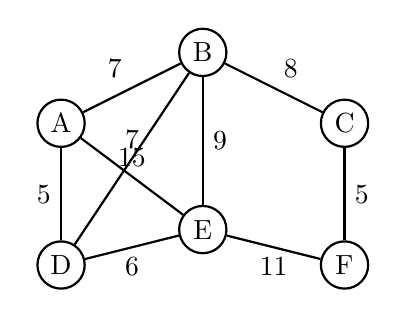
\begin{tikzpicture}[
    vertex/.style={circle, draw, minimum size=6mm, inner sep=0pt},
    thick, scale=0.9
  ]
  \node[vertex] (A) at (0,2) {A};
  \node[vertex] (B) at (2,3) {B};
  \node[vertex] (C) at (4,2) {C};
  \node[vertex] (D) at (0,0) {D};
  \node[vertex] (E) at (2,0.5) {E};
  \node[vertex] (F) at (4,0) {F};
  \draw (A) -- node[above left] {7} (B);
  \draw (A) -- node[left] {5} (D);
  \draw (B) -- node[above right] {8} (C);
  \draw (B) -- node[right] {9} (E);
  \draw (C) -- node[right] {5} (F);
  \draw (D) -- node[below] {6} (E);
  \draw (E) -- node[below] {11} (F);
  \draw (A) -- node[above] {15} (E);
  \draw (B) -- node[above] {7} (D);
\end{tikzpicture}
\end{center}
\end{exercise}

\begin{exercise}[$\star\star\star$ -- PERT/CPM]
A project has the following tasks:
\begin{center}
\begin{tabular}{cccc}
  \toprule
  Task & Duration & Predecessors \\
  \midrule
  A & 3 & -- \\
  B & 5 & A \\
  C & 2 & A \\
  D & 4 & B, C \\
  E & 6 & C \\
  F & 2 & D, E \\
  \bottomrule
\end{tabular}
\end{center}
Build the project graph, find the critical path and the minimum project
duration.
\end{exercise}
